\documentclass[11pt,preprint, authoryear]{elsarticle}

\usepackage{lmodern}
%%%% My spacing
\usepackage{setspace}
\setstretch{1.2}
\DeclareMathSizes{12}{14}{10}{10}

% Wrap around which gives all figures included the [H] command, or places it "here". This can be tedious to code in Rmarkdown.
\usepackage{float}
\let\origfigure\figure
\let\endorigfigure\endfigure
\renewenvironment{figure}[1][2] {
    \expandafter\origfigure\expandafter[H]
} {
    \endorigfigure
}

\let\origtable\table
\let\endorigtable\endtable
\renewenvironment{table}[1][2] {
    \expandafter\origtable\expandafter[H]
} {
    \endorigtable
}


\usepackage{ifxetex,ifluatex}
\usepackage{fixltx2e} % provides \textsubscript
\ifnum 0\ifxetex 1\fi\ifluatex 1\fi=0 % if pdftex
  \usepackage[T1]{fontenc}
  \usepackage[utf8]{inputenc}
\else % if luatex or xelatex
  \ifxetex
    \usepackage{mathspec}
    \usepackage{xltxtra,xunicode}
  \else
    \usepackage{fontspec}
  \fi
  \defaultfontfeatures{Mapping=tex-text,Scale=MatchLowercase}
  \newcommand{\euro}{€}
\fi

\usepackage{amssymb, amsmath, amsthm, amsfonts}

\def\bibsection{\section*{References}} %%% Make "References" appear before bibliography


\usepackage[round]{natbib}

\usepackage{longtable}
\usepackage[margin=2.3cm,bottom=2cm,top=2.5cm, includefoot]{geometry}
\usepackage{fancyhdr}
\usepackage[bottom, hang, flushmargin]{footmisc}
\usepackage{graphicx}
\numberwithin{equation}{section}
\numberwithin{figure}{section}
\numberwithin{table}{section}
\setlength{\parindent}{0cm}
\setlength{\parskip}{1.3ex plus 0.5ex minus 0.3ex}
\usepackage{textcomp}
\renewcommand{\headrulewidth}{0.2pt}
\renewcommand{\footrulewidth}{0.3pt}

\usepackage{array}
\newcolumntype{x}[1]{>{\centering\arraybackslash\hspace{0pt}}p{#1}}

%%%%  Remove the "preprint submitted to" part. Don't worry about this either, it just looks better without it:
\makeatletter
\def\ps@pprintTitle{%
  \let\@oddhead\@empty
  \let\@evenhead\@empty
  \let\@oddfoot\@empty
  \let\@evenfoot\@oddfoot
}
\makeatother

 \def\tightlist{} % This allows for subbullets!

\usepackage{hyperref}
\hypersetup{breaklinks=true,
            bookmarks=true,
            colorlinks=true,
            citecolor=blue,
            urlcolor=blue,
            linkcolor=blue,
            pdfborder={0 0 0}}


% The following packages allow huxtable to work:
\usepackage{siunitx}
\usepackage{multirow}
\usepackage{hhline}
\usepackage{calc}
\usepackage{tabularx}
\usepackage{booktabs}
\usepackage{caption}


\newenvironment{columns}[1][]{}{}

\newenvironment{column}[1]{\begin{minipage}{#1}\ignorespaces}{%
\end{minipage}
\ifhmode\unskip\fi
\aftergroup\useignorespacesandallpars}

\def\useignorespacesandallpars#1\ignorespaces\fi{%
#1\fi\ignorespacesandallpars}

\makeatletter
\def\ignorespacesandallpars{%
  \@ifnextchar\par
    {\expandafter\ignorespacesandallpars\@gobble}%
    {}%
}
\makeatother

\newlength{\cslhangindent}
\setlength{\cslhangindent}{1.5em}
\newenvironment{CSLReferences}%
  {\setlength{\parindent}{0pt}%
  \everypar{\setlength{\hangindent}{\cslhangindent}}\ignorespaces}%
  {\par}


\urlstyle{same}  % don't use monospace font for urls
\setlength{\parindent}{0pt}
\setlength{\parskip}{6pt plus 2pt minus 1pt}
\setlength{\emergencystretch}{3em}  % prevent overfull lines
\setcounter{secnumdepth}{5}

%%% Use protect on footnotes to avoid problems with footnotes in titles
\let\rmarkdownfootnote\footnote%
\def\footnote{\protect\rmarkdownfootnote}
\IfFileExists{upquote.sty}{\usepackage{upquote}}{}

%%% Include extra packages specified by user

%%% Hard setting column skips for reports - this ensures greater consistency and control over the length settings in the document.
%% page layout
%% paragraphs
\setlength{\baselineskip}{12pt plus 0pt minus 0pt}
\setlength{\parskip}{12pt plus 0pt minus 0pt}
\setlength{\parindent}{0pt plus 0pt minus 0pt}
%% floats
\setlength{\floatsep}{12pt plus 0 pt minus 0pt}
\setlength{\textfloatsep}{20pt plus 0pt minus 0pt}
\setlength{\intextsep}{14pt plus 0pt minus 0pt}
\setlength{\dbltextfloatsep}{20pt plus 0pt minus 0pt}
\setlength{\dblfloatsep}{14pt plus 0pt minus 0pt}
%% maths
\setlength{\abovedisplayskip}{12pt plus 0pt minus 0pt}
\setlength{\belowdisplayskip}{12pt plus 0pt minus 0pt}
%% lists
\setlength{\topsep}{10pt plus 0pt minus 0pt}
\setlength{\partopsep}{3pt plus 0pt minus 0pt}
\setlength{\itemsep}{5pt plus 0pt minus 0pt}
\setlength{\labelsep}{8mm plus 0mm minus 0mm}
\setlength{\parsep}{\the\parskip}
\setlength{\listparindent}{\the\parindent}
%% verbatim
\setlength{\fboxsep}{5pt plus 0pt minus 0pt}



\begin{document}



\begin{frontmatter}  %

\title{Cross Section Project: Difference-in-Difference Analysis}

% Set to FALSE if wanting to remove title (for submission)




\author[Add1]{Samantha Scott}
\ead{20945043@sun.ac.za}





\address[Add1]{Stellenbosch University, Cape Town, South Africa}

\cortext[cor]{Corresponding author: Samantha Scott}


\vspace{1cm}


\begin{keyword}
\footnotesize{
Difference-in-difference analysis \sep PIRLS data \sep Child Support
Grant \\
\vspace{0.3cm}
}
\end{keyword}



\vspace{0.5cm}

\end{frontmatter}



%________________________
% Header and Footers
%%%%%%%%%%%%%%%%%%%%%%%%%%%%%%%%%
\pagestyle{fancy}
\chead{}
\rhead{}
\lfoot{}
\rfoot{\footnotesize Page \thepage}
\lhead{}
%\rfoot{\footnotesize Page \thepage } % "e.g. Page 2"
\cfoot{}

%\setlength\headheight{30pt}
%%%%%%%%%%%%%%%%%%%%%%%%%%%%%%%%%
%________________________

\headsep 35pt % So that header does not go over title




\newpage

\hypertarget{introduction}{%
\section{Introduction}\label{introduction}}

The following paper is an investigation of the Child Support Grant (CSG)
and its impact on learning outcomes in South Africa. More specifically,
this paper aims to estimate the effect that broader eligibility criteria
would have on reading outcomes of grade 4 learners between the years
2011 and 2016. The broader criteria was a result of an increase in age
eligibility of children to under 18 years of age in 2012. To investigate
the causal effect of this policy change on the reading scores of
children, a difference-in-difference estimation is conducted. In the
estimation, individuals who qualified for the grant in their respective
years are described as the treatment group, whereas the individuals who
lie above the threshold are described as the control group. This paper
uses the Progress in International Reading Literacy Study (PIRLS) data
for 2011 and 2016 to investigate the research question at hand, and
although the investigation is subject to limitations, the results are
still noteworthy. The paper concludes that the policy change, namely the
rise in age eligibility, has positively affected the learning scores of
the treatment group.

\hypertarget{difference-in-differnce-estimation}{%
\section{Difference-in-Differnce
Estimation}\label{difference-in-differnce-estimation}}

Difference-in-difference methods are widely used in the field of
Economics to conduct policy evaluation with observational data
(Sant'Anna \& Zhao 2020:101-102). A difference-in-difference estimation
makes use of the outcome of a control group as a proxy for the outcome
for the treatment group, if the treatment had not occurred. This method
requires there to be a treatment group, who is not treated in period one
but treated in period two, as well as a control group who is not treated
in either period. To obtain the difference-in-difference estimate, it is
required to obtain the difference in before and after the treatment for
the treated, and the control (untreated) group. The difference between
these two differences is known as the difference-in-difference estimate,
which is depicted in mathematical form below:

\[ \rho = (Y_{treated2016} - Y_{treated2011}) - (Y_{untreated2016} - Y_{untreated2011})\]

\hypertarget{data-and-methodology}{%
\section{Data and Methodology}\label{data-and-methodology}}

According to previous literature, there was an increase in the maximum
income per caretaker per annum between 2011 and 2016, which could have
resulted in an increase in the eligibility of the caretakers in the
population. After 2008, the threshold placed on the national income per
caretaker per annum by the government was R27 600 (Beukes, Jansen,
Moses, \& Yu, 2017:513). By 2016, this threshold rose to R39 600 per
caretaker per annum to qualify for the grant (Bhorat \& Köhler,
2020:23). According to Statistics South Africa, expenditure per
household in 2011 and 2016 for quintile two was R32 569 and R43 452,
respectively (Statistics South Africa, 2015:) \& (Statistics South
Africa, 2017:). Although there was an increase in the threshold amount,
the jump was not large enough for another quintile to qualify.
Therefore, for this investigation, the treatment group in both 2011 and
2016 is quintile one.According to Beukes et al.~(2017:513), the
eligibility criteria that qualified mothers for the CSG became broader
in 2012. This was due to a rise of the maximum age the child could be
for the mother to be eligible. The increase in age was up to 18 years of
age. This increase in the number of individuals eligible for the CSG may
result in an improvement of learning outcomes, for example, reading
outcomes. To investigate this research question, the data used is the
Progress in International Reading Literacy Study (PIRLS) for South
Africa in 2011 and 2016. The samples are made of 12 810 grade 4 learners
and are assessments of reading comprehension of the learners. In 2011,
the sample was nationally representative, but was only stratified by
language. In 2016, the sample was also nationally representative, but
was stratified by both language and province (Howie, Combrinck, Roux,
Tshele, Mokoena, \& McLeod Palane, 2017:2).

To approximate wealth for the creation of the treatment group, the
possessions that learner's indicated having in their homes are used. In
doing so, an asset index of wealth is created. From this variable, a
peer quintile variable is formulates,distinguishing between the
different wealth groups of the population. Using these quintiles, it may
be assessed whether an individual would have qualified for the CSG in
2011, and in 2016. If they qualified for the grant, the individuals are
described as the treatment group. The individuals who fall above the
threshold, are described as the control group. Using the treatment
variable described above, an OLS regression is run to estimate the
effect of the quintile the child falls under on their reading outcomes.
In this first model, the learner's age and gender is included. A simple
difference-in-difference regression is then run. The model includes only
the treatment and control groups, the year before and after treatment,
as well as the interaction term of the year after treatment and the
treated. The third and fourth models introduce controls to the simple
difference-in-difference estimation. The controls that are added is the
learner's age and gender.

\hypertarget{results-and-discussion}{%
\section{Results and Discussion}\label{results-and-discussion}}

In Figure 4.1 below, model (1) is an OLS regression. In this model, the
coefficient on the treatment group is negative. This is because the
model is estimating the effect of the learner being in quintile one on
their reading outcomes. As such, the coefficient on treatment group does
not provide an accurate view of impact of the policy change on the
treatment group. The coefficient on the learner's age is also negative.
This is because PIRLS assesses grade 4 learners. If a child is older
than 10 years of age, it means the child could have either failed one or
more years. This may be indicative of the child's lower learning
ability. By controlling for gender in this model, it is evident that
girls have higher reading scores than boys. Although controls have been
added to the model, there may still be unobservables in the error term
which may bias the coefficient on the learner's quintile.

In the figure, model (2) is a simple difference-in-difference
estimation. This model indicates that there is a positive effect of the
broader eligibility criteria of the CSG that was implemented in 2012 on
the treatment group. This method allows a better understanding of the
impact of the policy change on the affected group, as opposed to the OLS
regression. In checking the robustness of the results from model (2),
controls are added to the simple difference-in-difference estimation. In
model (3), the learner's age is added. As a result, the coefficient on
the interactive term remains positive, but slightly decreases. When
another variable is added, namely gender, in model (4), the coefficient
drops slightly more, but still remains positive. This indicates that the
strength of the effect is not accurate, however, the direction of the
effect is accurate.

\begin{figure}
\centering
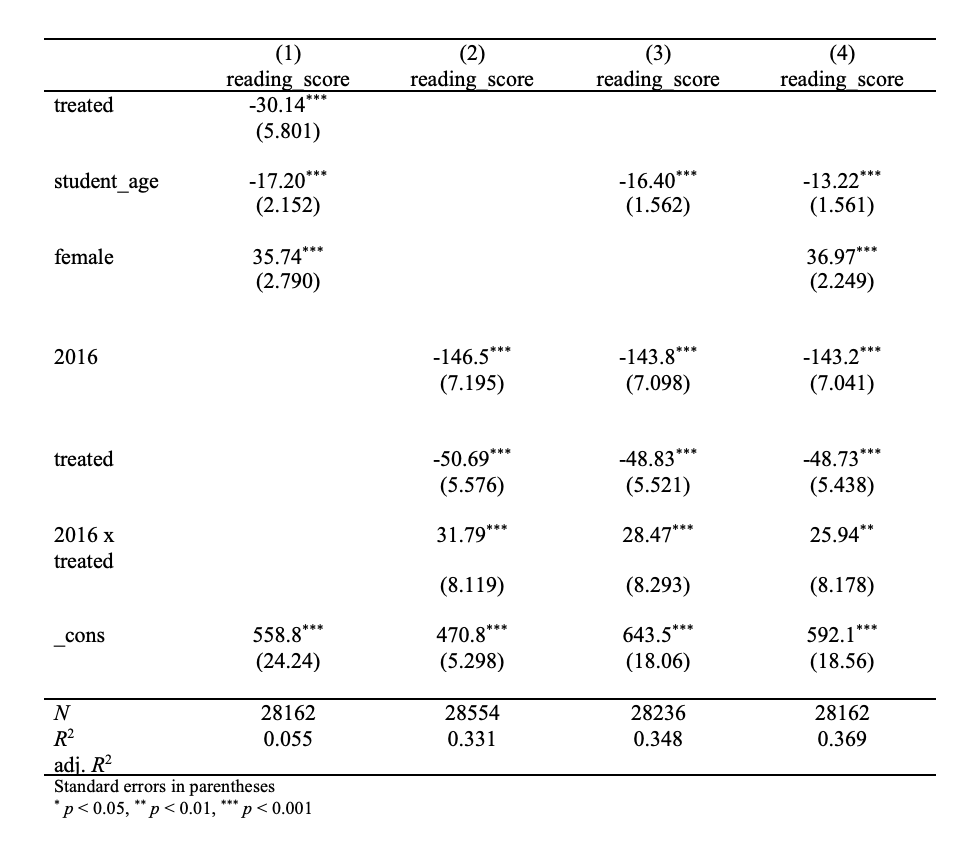
\includegraphics[width=\textwidth,height=0.65\textheight]{/Users/samanthascott/Desktop/CS_proj/reg.png}
\caption{Regression Table}
\end{figure}

Figure 4.2 depicts the decrease in reading scores from 2011 to 2016, for
the control group as well as the treatment group. As seen in the figure
below, the reading scores for the control group are greater than those
of the treatment group in both 2011 and 2016. However, the decrease in
reading scores for the control group is larger than that of the the
treatment group. Figure 4.2 therefore justifies the positive result
presented by the difference-in-difference estimations, as the difference
between the differences in treated and in untreated would be positive.

\begin{figure}
\centering
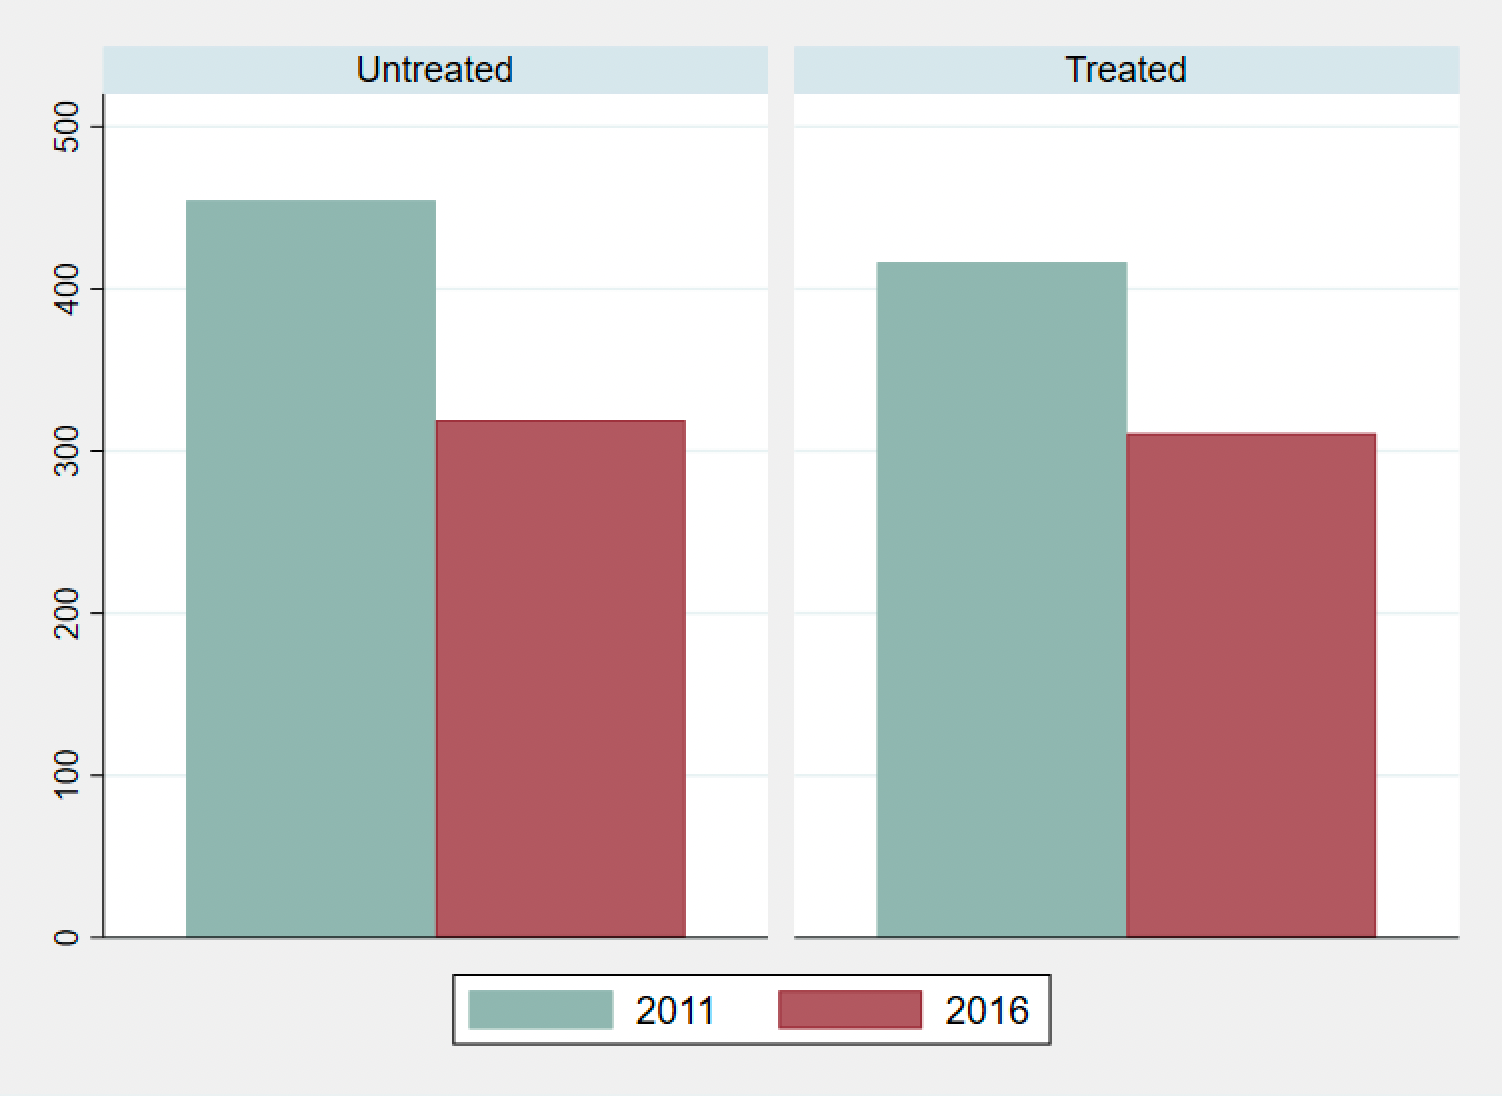
\includegraphics[width=0.7\textwidth,height=0.4\textheight]{/Users/samanthascott/Desktop/CS_proj/bar.png}
\caption{Reading Scores: Untreated vs.Treated}
\end{figure}

Figures 4.3 and 4.4 depict the reading scores per quintile in 2011 and
2016, respectively. As seen in the graphs below, the reading scores of
the population drops over all quintiles. This indicates that the drop in
reading scores for quintile one is not unique to the rest of the
population. Using the graphs below, it is evident that the percentage
change of the mean of reading scores between 2011 and 2016 is the lowest
for quintile one in comparison to the other quintiles, as the difference
in the average reading score of quintile one between 2011 and 2016 is
105. This value increases for each quintile.

\begin{figure}
\centering
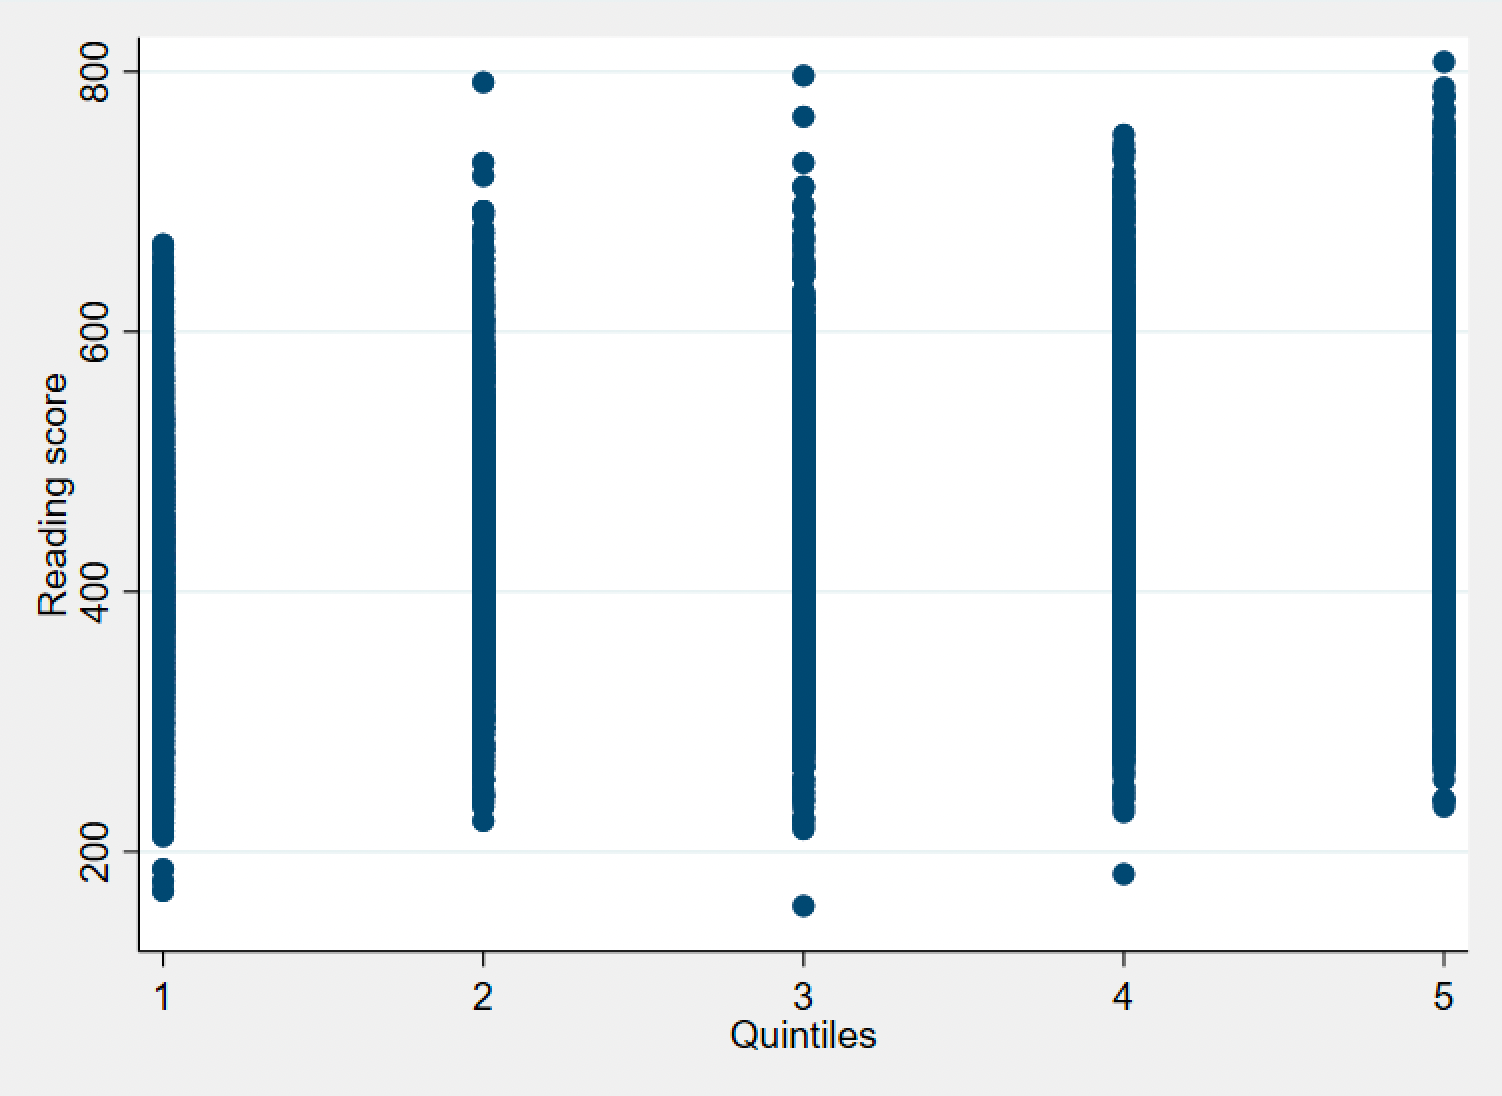
\includegraphics[width=0.6\textwidth,height=0.3\textheight]{/Users/samanthascott/Desktop/CS_proj/2011scatter.png}
\caption{Reading Scores per Quintile in 2011}
\end{figure}

\begin{figure}
\centering
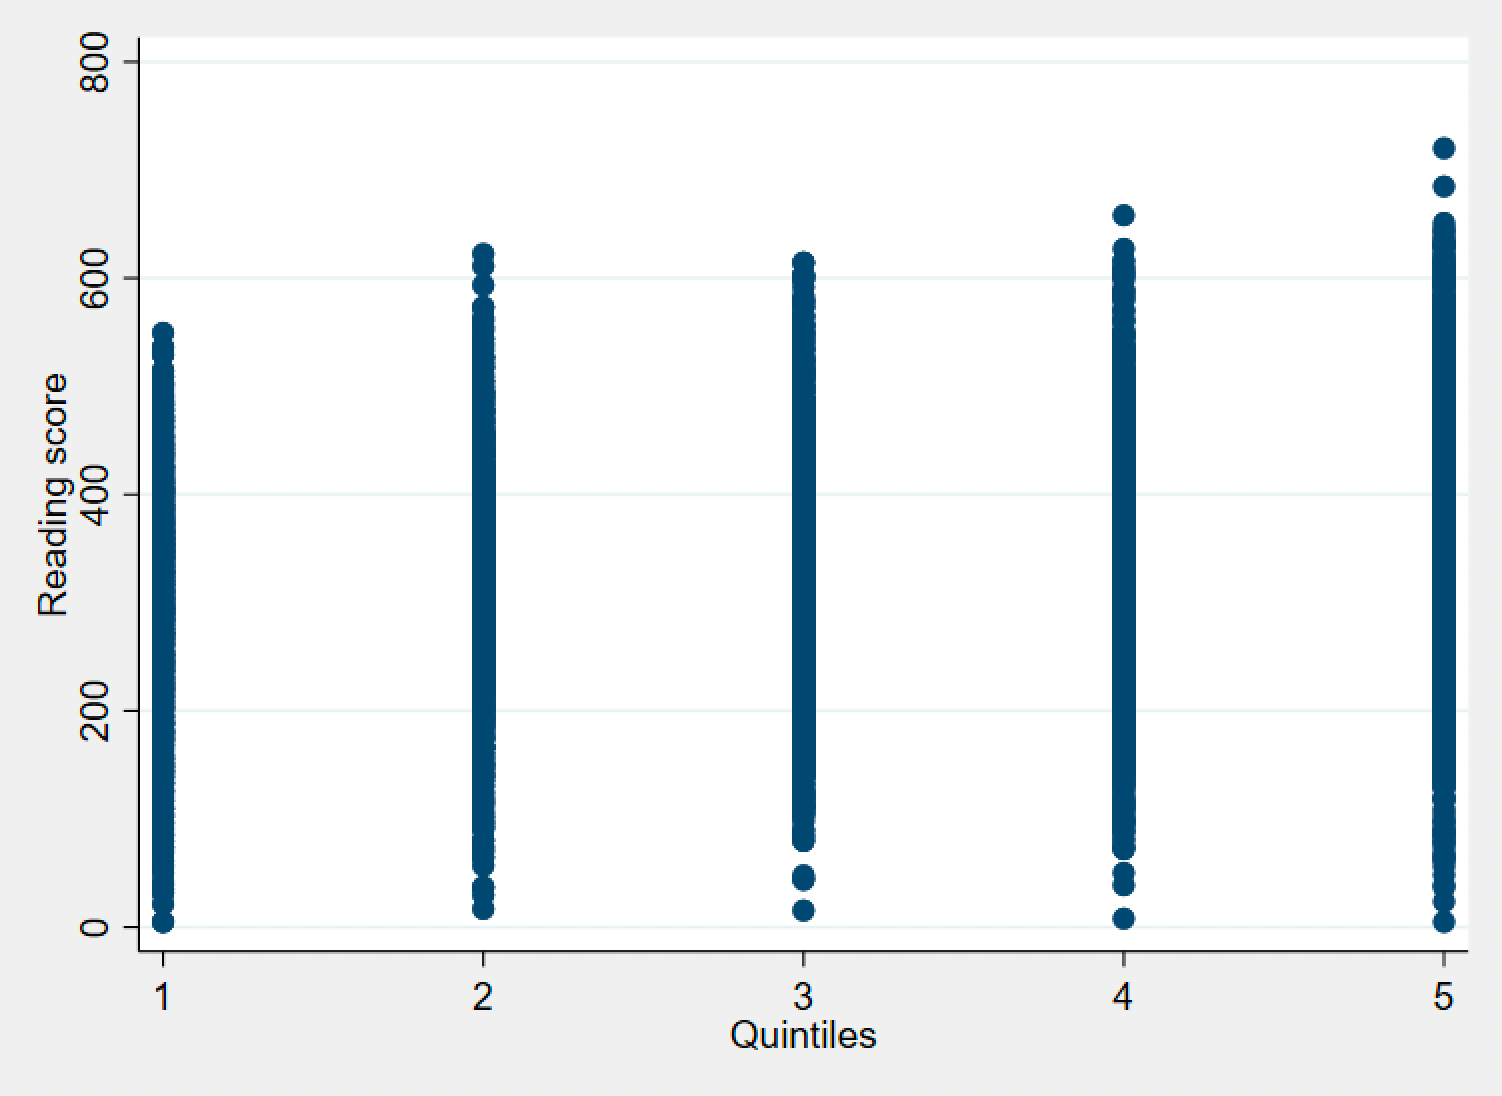
\includegraphics[width=0.6\textwidth,height=0.3\textheight]{/Users/samanthascott/Desktop/CS_proj/2016scatter.png}
\caption{Reading Scores per Quintile in 2016}
\end{figure}

\hypertarget{limitations}{%
\section{Limitations}\label{limitations}}

In this investigation, several limitations are evident. This first
limitation is that in the PIRLS 2011 and 2016 datasets, there are no
variables indicative of household or parental income levels. In order to
develop a measure of wealth, an asset index is created. By using an
asset index to determine the treatment group, there is room for error.
The wealth measure is presented in quintiles, which when converted to
income levels using external data, provides a range of income levels. As
such, it is not possible to create an accurate representation of the
treatment group.

The next limitation is that there are no variables that indicate if an
individual has received a grant in the data. In this investigation, it
is assumed that if individuals qualified for the grant, they received
the grant. The problem with the intention to treat is that the
individuals are not necessarily offered the grant and declining to
receive it. There are costs involved with obtaining the grant, which may
hinder individuals from receiving it. Another limitation of this
investigation is that variable indicating the race of a learner is not
included in the data. This is problematic when developing the models as
the race of a student is likely to affect the learning outcomes of the
learner, due to South Africa's apartheid history which has resulted in
systematic issues that need to be accounted for in the models.

\hypertarget{conclusion}{%
\section{Conclusion}\label{conclusion}}

In conclusion, through conducting a difference-in-difference analysis of
PIRLS 2011 and 2016 data, it is evident that the rise in eligibility of
Child Support Grant (CSG) recipients due to an increase in maximum age
has resulted in a positive effect on the reading scores of grade 4
learners in South Africa. Through the addition of controls to the simple
difference-in-difference estimation, the direction of the positive
effect of the policy change on reading scores is robust. When the data
is investigated further, it is evident that although the overall reading
scores of the population dropped from 2016 to 2011, the drop in the
treatment group was smaller than that of the untreated group. This
reinforces the results of the difference-in-difference estimation. The
investigation is faced with several limitations, such as the neglect of
variables that hold important information for the question at hand (for
example, a grant recipient variable), however the results are still
noteworthy.

\newpage

\hypertarget{reference-list}{%
\section{Reference List}\label{reference-list}}

Beukes, R., Jansen, A., Moses, M. \& Yu, D. 2017. Exploring the
Eligibility Criteria of the Child Support Grant and its Impact on
Poverty. \emph{Social Indicators Research}, 134:511-529.

Bhorat, H. \& Köhler, T. 2020. Social Assistance during South Africa's
National Lockdown: Examining the COVID-19 grant, changes to the Child
Support Grant and post-October policy options. \emph{Development Policy
Research Unit.} Working Paper No.~202009.

Gerwyn, N. 2019. \emph{Generalised Regression Difference in Differences:
with Fixed Effects, Multiple Treatment Periods and Dynamic Treatment
Effects} {[}Online{]}. Available:
\url{https://medium.com/eatpredlove/regression-difference-in-differences-208c2e787fd2}
{[}2022, 19 June{]}.

Howie, S.J., Combrinck, C., Roux, K., Tshele, M., Mokoena, G.M., \&
McLeod Palane, N. (2017). \emph{PIRLS LITERACY 2016: South African
Highlights Report.} Pretoria: Centre for Evaluation and Assessment.

Sant'Anna, P. \& Zhao, J. 2020. Doubly Robust Difference-in-Differences
Estimators. \emph{Journal of Econometrics}, (219):101-122.

Statistics South Africa. 2015. Earnings and Spending in South Africa,
2006--2011.

Statistics South Africa. 2017. Living Conditions of Households in South
Africa.

\bibliography{Tex/ref}





\end{document}
